\chapter{Theory: How to calculate grating efficiency}
\section{Introduction to grating theory}
\begin{figure}[htbp] %  figure placement: here, top, bottom, or page
   \centering
   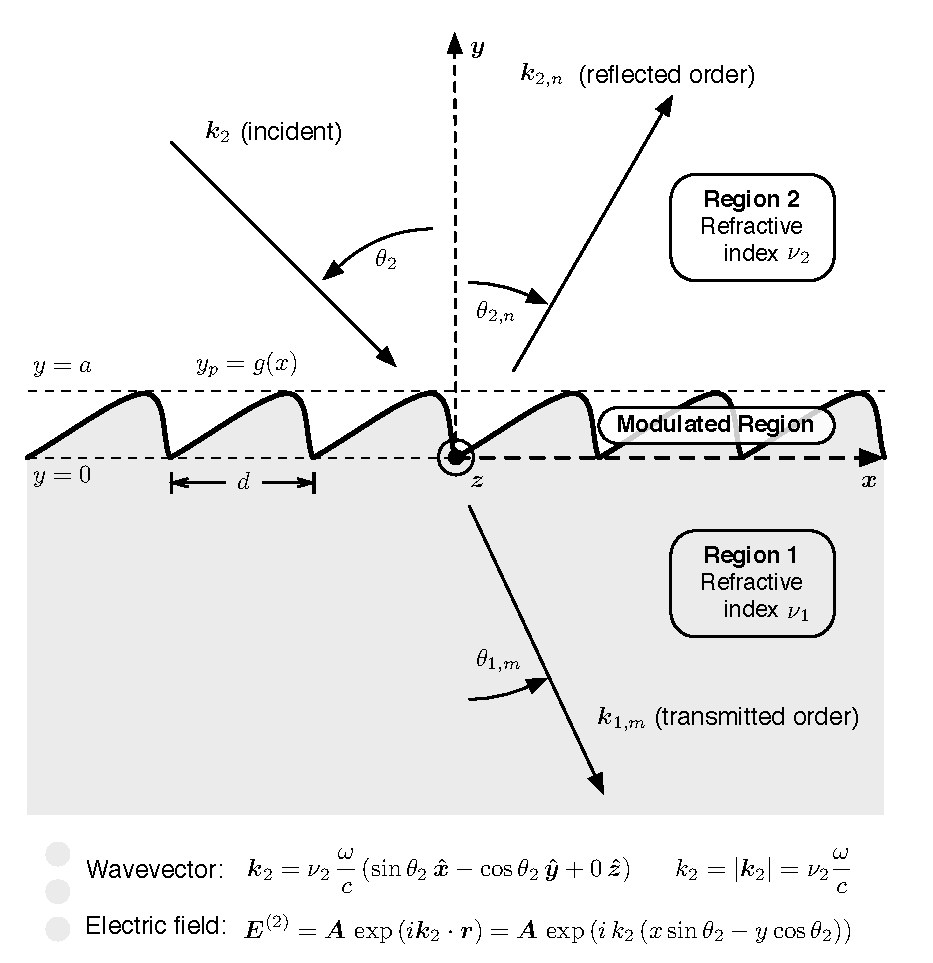
\includegraphics[scale=0.8]{Chapter2/2a_inPlaneIncidence/2a.pdf} 
   \caption{A one-dimensional grating with in-plane incidence.}
   \label{2a}
\end{figure}

For centuries, we have known that gratings reflect and transmit light at a set of discrete angles -- called \emph{orders} -- where the angles depend on the wavelength  (Figure \ref{2a}).  A variety of simple proofs have been used to explain this.  In undergraduate books, the grating equation is introduced as a consequence of constructive interference from a linear array of coherent emitters. (This makes sense for a slotted transmission grating, but it is less obvious why an arbitrarily-shaped periodic structure like one of those shown in Figure \ref{3c-profile} would behave the same way.)  Other proofs -- such as those using Fermat's Principle to minimize an optical path function with a phase offset introduced by the grating \cite[p.~93 -- 99]{Pea97} -- are general enough to explain the existence of diffraction orders, but they do not say anything about how much light goes into each.

This is unfortunate, because to determine grating efficiency, we must determine the intensity of the orders.  A huge amount of research has gone into this question since Lord Rayleigh's pioneering work in 1907 \cite{Ray07}, and some clever analytical methods were even discovered that simplify the problem -- but only for certain special groove shapes.  It is only within the last twenty years that mathematical techniques and computational power have advanced enough to accurately model the electromagnetic field of light within and near the surface of an arbitrary grating, allowing us to actually determine how energy is distributed between the orders, and how much is absorbed within the grating.  In this chapter, we look at a history of the key developments in grating theory, give a comparison of the current methods, and then set up the grating problem using the most general of these methods.

\subsection{A brief history of grating theory}

The ``grating problem'' -- as we define it -- is the problem of determining the intensity of a grating's reflected and transmitted light everywhere.  In general, this requires finding the solution to Maxwell's equations for the electric and magnetic fields of the light, in the presence of the grating's periodic boundary conditions, for a known incident field.  

Prior to the availability of computers and numerical techniques, great attempts were made to solve this problem analytically.  In 1907, Lord Rayleigh set up the problem\footnote{Actually, Rayleigh's first application of this technique was to the diffraction of sound waves \cite{Ray86}.  It turns out that the wave equation for a pressure wave in compressible media is the same as for the fields in an electromagnetic wave, and the boundary conditions at interfaces are also analogous. In Ref. \cite{Ray07} he shows applications to both sound and light.} using a Fourier approach identical to the one we use later in this chapter \cite{Ray07}.  However, without access to powerful numerical methods, he could only make coarse approximations, using expansions truncated at the first or second power of the groove height.\footnote{And this, despite assuming a perfectly reflecting grating, exactly normal incidence, and only one term in the Fourier expansion for the groove shape -- i.e., a sinusoidal grating.}  This led to some obviously non-physical results, such as predictions of infinite intensity in any order when the outgoing angle of a higher order reached exactly 90 degrees.  From 1907 until 1960, advancements in grating theory amounted to finding clever but limited simplifications to these expansions, which would work in the case of one particular groove profile, incidence angle, or approximation limit.

The introduction of computer-based numerical methods in the 1960s spawned a renewal of research into general solutions to the problem.  The first ``rigorous'' algorithm\footnote{``Rigorous'' meaning a method that does not introduce approximations into the theoretical equations, other than inevitably in the process of finite-precision numerical calculations.} was invented by several researchers in 1966:
\begin{description}
\item[The ``integral'' approach] uses Maxwell's equations in integral form and the Kirchoff integral theorem \cite{Pet66}\cite{Wir69}\cite{Pav70}.  It was generalized from perfectly conducting (i.e.: perfectly reflecting) gratings to finite-conductivity metallic gratings in an important paper in 1972 \cite{May72}.
\end{description}
Alongside these ``integral'' methods, two other broad families of algorithms emerged based on Maxwell's equations in differential form:
\begin{description}
\item[The ``modal'' method] relates the electromagnetic field to a Fourier expansion in the vertical ($y$) direction with unknown coefficients, called modes. The total field satisfying the boundary conditions is solved algebraically as a linear combination of the modes \cite{Bot81}\cite{Bot81a}\cite{And81}.
\item[The ``differential'' methods] exploit the periodicity of the grooves to express both the grating boundary and the fields as Fourier expansions in the $x$-direction. The total field satisfying the boundary conditions is determined by numerically integrating a finite set of differential equations. (We explore the details of this method later in this chapter.)
\end{description}
The modal methods are not actually general because in their application of the boundary conditions, they require the edges of the grooves to be vertical; this limits them to rectangular gratings.
%they are accurate in this special case, and fast compared to the differential method because they avoid numerical integration.  
The other two approaches are general in representation, although the integral approach can only be solved for certain geometries.

By 1980, grating theorists had devised a wide variety of implementations for each family.  % -- after all, it is one matter to express the problem as a complete set of algebraic or differential equations; it is another matter to actually solve that set!
Reference \cite{Pet80} provides a comprehensive review of all the methods that were available by this date.\footnote{The same author provides a follow-up paper, written ten years later on new methods that differ completely from the fundamentals used in 1980 \cite{Pet90}.}  Of the three families, the differential approach had proven to be the most general way of setting up the problem, but it ran into two numerical issues -- particularly when used to describe TM-polarized light on highly-conducting metallic gratings.  One issue was strictly computational: round-off errors when doing finite-precision computer arithmetic would lead to ever-growing contamination during the numerical integration of exponential functions.  This problem was solved by the introduction of the ``S-matrix'' propagation algorithm in 1996 \cite{Li96}\cite{Mon98}.  The second problem was related to the mathematical implications of truncating an infinite Fourier series -- unfortunately but obviously necessary for numerical calculations.  This challenge was also finally resolved by the breakthrough work of Li \cite{Li96b} in 1996 on the factorization of truncated Fourier series, and has been applied extensively by Neviere and Popov both to the simple cases of one-dimensional gratings like those shown in Figure \ref{2a} \cite{Pop01}, and to complex three-dimensional periodic structures of anisotropic materials \cite{Pop00}\cite{Nev02}.

\subsection{Comparison and applicability of grating theory families}
To choose an appropriate method for a particular problem, we need to understand the assumptions and limitations of each one.  This section presents just enough theory to understand their areas of applicability.
\subsubsection{The Integral Method}
For a perfectly conducting metal, when an electromagnetic is incident on the surface, it will induce a surface current $\mathbf{j}_S(\mathbf{M}')$ at each point $\mathbf{M}'$.  This surface current radiates a field -- the diffracted electric field $E(P)$ at a given point $\mathbf{P}$ above the surface; the field is related to the surface current by the Kirchoff Integral Theorem \cite{Kir83} using the Green's function $G(\mathbf{P}, \mathbf{M}')$:
\begin{eqnarray}
\mathbf{E}(\mathbf{P}) = \int\limits_{\textrm{grating period}} G(\mathbf{P}, \mathbf{M}')\, \phi(\mathbf{M}')\, \dif s'
\end{eqnarray}
where $\dif s$ is a curvilinear coordinate along the grating profile, and $\phi(\mathbf{M'})$ is proportional to the surface current.  Unfortunately, this becomes tricky, because the surface current is not only induced by the incident electric field, but also by the diffracted field radiated from all other points along the grating surface.  This means that the surface current $\mathbf{j}_S(\mathbf{M}')$ at $\mathbf{M}'$ depends not on the incident field, but also on the current $\mathbf{j}_S(\mathbf{M}'')$ at all coordinates $\mathbf{M}''$.  By substituting the corresponding $\phi(\mathbf{M'})$ into the equation above, this transforms it into not a differential equation, but an integral equation for $\phi(\mathbf{M'})$.  

\noindent\textbf{\emph{Limitations}}\\
In practice, the numerical techniques required to solve this integral equation can be complicated, depending on the shape of the profile.  For imperfectly-conducting gratings, the problem becomes even more difficult, and even harder still when the grating is made up of one or many layers -- such as over-coated soft x-ray gratings and multilayers.  Although it is universal, the main limitation of the integral approach is its computational cost, and the programming difficulty of applying it correctly to every unique grating situation; numerical challenges abound, particularly regarding the discretization of the grating profile and how sharp corners and discontinuities are handled.  Reference \cite{Pom91} presents an overview of integral implementations, as well as approximations for reducing the computation time and handling coating layers. The latest version -- referred to as the ``modified integral method'' by Goray, has been the topic of many recent publications \cite{Gor02} \cite {Gor02b} \cite{See02} \cite{Gor05}.

\subsubsection{Methods using Maxwell's Equations in differential form}
The remaining two families (the modal method and the differential method) start from Maxwell's equations in differential form.  Within the differential method, there are two variants: the ``classical'' differential method, and the ``Rigorous Coupled Wave'' (RCW) approach.  We present all three here together because they share the same foundation.  They all start by projecting the solution to Maxwell's Equations -- i.e., the strength of the electric or magnetic field of the waves -- onto some periodic basis in the $x$-direction, but with an unknown dependence on $y$.  The task for each method is to determine the $y$-dependence by ensuring the total field satisfies the boundary conditions on the grating surface and at infinite.  The modal method and the RCW method both assume a rectangular groove profile, so that the boundary conditions are simplified: this implies that the tangential and normal field components at the grating interface are purely along either the $x$ or $y$-direction.
\begin{description}
\item[The modal method] assumes a basis of functions that are periodic in $x$, with ``modes'' $F_m$ related to the field $u_m(x)$ as
\begin{eqnarray}
F_m(x,y)=u_m(x) \, \exp \left( i \rho_m y \right)
\end{eqnarray}
where $\rho_m$ is a ``mode constant''.  The total field is assumed to be a linear combination of the modes with unknown amplitudes, and since this field must satisfy the boundary conditions on the surface, it is possible to create a set of linear algebraic equations which can be solved for the mode amplitudes.

\noindent\textbf{\emph{Limitations}}\\
For the modal method, the number of modes and the mode constants $\rho_m$ must be sufficient to fully describe the actual field.  For highly conducting materials, finding appropriate mode constants is difficult, but a technique is available in Ref. \cite{And81}.  

The other obvious limitation of the modal method is to rectangular gratings with vertical groove boundaries.  We can attempt to avoid this limitation by using stacks of thin rectangular gratings to represent an arbitrary shape, as we will see in Section \ref{stacksOfGratings}.  This is called the ``staircase approximation'' for obvious reasons, and is also used in the RCW method.  Unfortunately, no matter how thin the slices are made, this approximation creates sharp edges between the layers at the stair-step corners.  Popov et. al. discovered that for TM-polarized light, this creates unrealistically strong electric fields at the corners, which cannot be physically representative of the true electric field near a smooth grating.  Therefore, algorithms that use the staircase approximation require a larger number of basis components to represent this abruptly changing field, which slows down the computation.  More importantly, even when there are enough components to let the solution converge, the results are not representative of reality. \cite{Pop02} 

\item[The differential method's ``classical solution''] uses a periodic field similar to the modal method, except that the basis functions are Fourier terms in the $x$-direction, and the unknown functions to solve are along the $y$-direction:
\begin{eqnarray}
F(x,y)=\exp\left( ik\, \sin \theta_{inc}x \right) \sum\limits_m F_m(y) \exp \left( \frac{2\pi i x}{d} \right)
\end{eqnarray}
By matching the total field to the boundary conditions at the top and bottom of the grooves, a set of coupled differential equations is created; this set is solved using a combination of numerical integration and linear algebra, which we describe later in this chapter.  

\noindent\textbf{\emph{Limitations}}\\
The advantage of the classical differential method is that it works for arbitrary groove profiles.  However, for rectangular profiles, it is slower than the other two options because of the necessity to perform a numerical integration for each basis component.  The pure differential method originally suffered from numerical convergence problems in TM polarization on conductive gratings, but these were resolved in 1995 \cite{Li96} \cite{Li96b} \cite{Pop00}.  The only remaining limitation is that the method assumes the material can be described by a well-behaved complex dielectric constant (or the related refractive index) both above and inside the grating material.  This rules out ``perfectly conducting'' (i.e., perfectly reflecting) gratings, for which it is not reasonable to assign a dielectric constant.  This limitation results in a numerical instability when trying to work with nearly perfectly conducting gratings -- for example, gold and aluminum metallic gratings used with deep infrared or millimetre light -- where the real part of the refractive index falls below 0.1.  (A few suggestions have been proposed recently for extending the differential method to highly conducting gratings, such as by substituting a finite-thickness perfectly-conducting layer above an absorbing substrate. \cite{Pop04})

\item[The differential method's ``Rigorous Coupled Wave'' approach] is a simplification that can be applied for rectangular gratings.  As we mentioned in the case of the modal method, when the groove edges are vertical, the boundary conditions within the grooves are invariant along the $y$-direction.  This means that an eigenvalue technique can be used instead of the full numerical integration along $y$, which reduces the problem to an algebraic solution, speeds up the calculation, and removes the numerical challenges associated with integrating growing exponentials.  As soon as this simplification was proposed, various authors \cite{Bur66} \cite{Pen75} \cite{Moh81} assumed that it could be generalized to arbitrary groove profiles by approximating them with rectangular slices, which could be made as thin as required for a given accuracy; this is the same ``staircase approximation'' used in the modal method.  The RCW approach was used extensively for thirty years, and has been shown to produce fast and accurate results for TE-polarized light on dielectric and absorbing gratings.  However, as we mentioned above, the fundamental validity of the staircase approximation was challenged in Ref. \cite{Pop02}.

\noindent\textbf{\emph{Limitations}}\\
As a differential method, the RCW approach is limited to finitely-conducting materials.  It is also limited to to rectangular gratings, or (using the staircase approximation) to stacks of rectangular layers in TE polarization; it can also produce approximate results in TM polarization for dielectric gratings.
\end{description}

Figure \ref{2e} gives a visual comparison of the limitations and strengths of all four techniques.

\begin{figure}[htbp] %  figure placement: here, top, bottom, or page
   \centering
   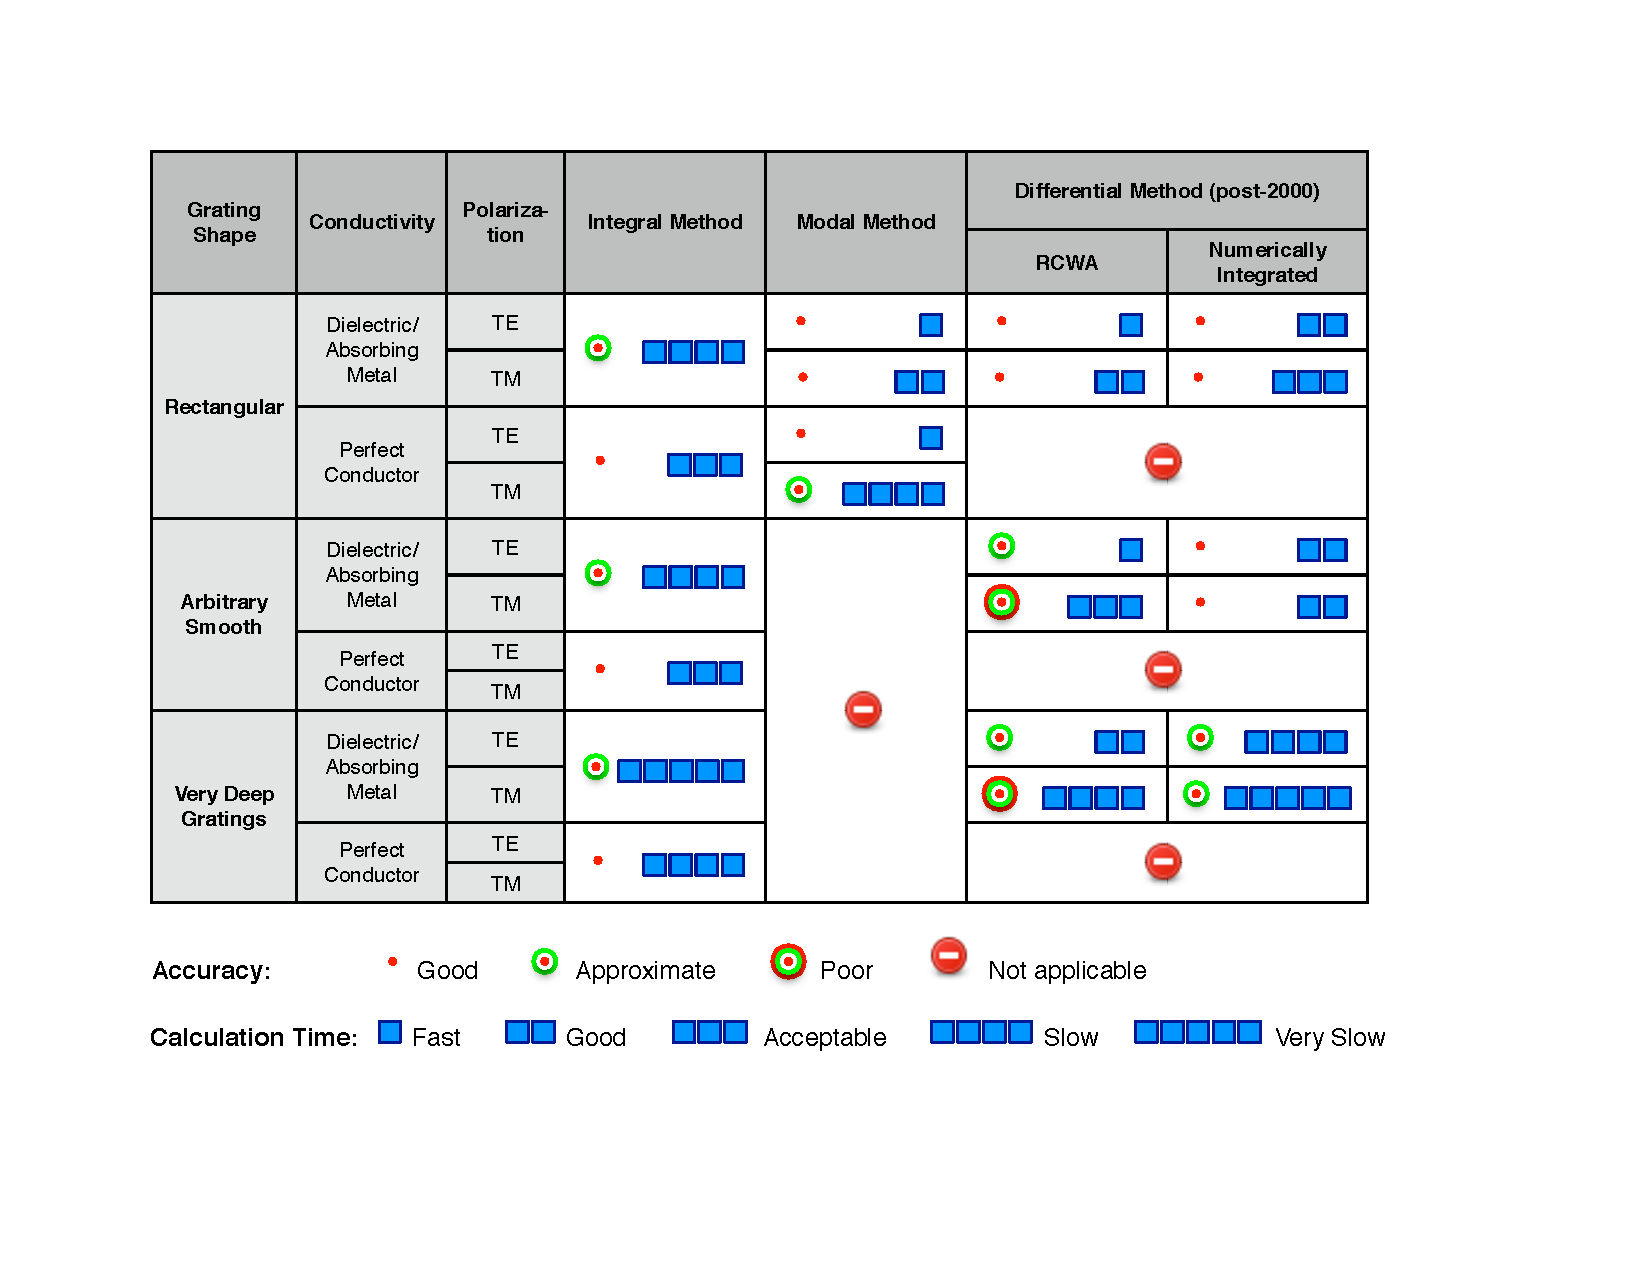
\includegraphics[scale=0.8]{../data/Chapter2/2e_methodComparision/methodComparisonTable_noPre2000.pdf} 
   \caption{A visual comparison of the limitations and strengths of the main methods in grating theory: the integral approach, the modal method, the full (numerically integrated) differential method, and differential method's ``RCW'' staircase-approximation simplification.}
   \label{2e}
\end{figure}


\subsubsection{Choosing a theoretical method}
Since we are primarily interested in the efficiency of soft x-ray gratings used in grazing incidence, the limitations we identified above provide clear guidance for choosing an appropriate method.  At the frequency of soft x-ray radiation, metals behave as absorbing, weak dielectrics with a refractive index near $(0.999 - 0.001i)$; therefore, we do not need to worry about limitations on perfectly-conducting materials.  At grazing incidence, polarization effects are also minimized; there turns out to be very little difference between measured and calculated results for TE and TM polarization.

We must be able to model a variety of groove profiles, including rectangular but also triangular, trapezoidal, and sinusoidal shapes, with at least one coating layer.  (The triangular, or ``blazed'' profile -- featuring sharp vertices -- will turn out to be particularly important; see Section \ref{gratingManufacturing}.)  Therefore, we ruled out the modal and RCW methods, and were left with a choice between the integral method and the full differential method.    Given the necessity of modelling coatings and sharp profiles, we selected the differential method for its simplicity and robustness.  We used an implementation of this method for all the grating efficiency calculations, optimizations, and comparisons shown later in this thesis.

\subsection{Overview of the differential theory}
The rest of this chapter lays the groundwork for a full electromagnetic theory describing the interaction of light waves with periodic structures.  The notation presented here is consistent with the notation used by Neviere in \cite{Nev02}.  However, before diving into the details of the mathematics, it might be useful to summarize the basic physical principles behind the solution:
  \begin{enumerate}
\item The theory starts by using the Maxwell equations to derive a 2nd-order wave equation for the electric and magnetic field of the light.  According to classical optics, the incoming light can be divided into two independent polarization components; the ``Transverse Electric'' (TE) component has its \emph{electric} field vector always parallel to the $z-$axis in Figure \ref{2a}, and the ``Transverse Magnetic'' (TM) component has its \emph{magnetic} field vector always parallel to the $z-$axis.  Due to the beautiful symmetry of the Maxwell equations, it turns out that the wave equation for the electric field in TE polarization is the same as the equation for the magnetic field in TM polarization, and for most of the theory we can use the same mathematics to work with both, referred to as the ``general field'' or just ``the field''.\footnote{While the wave equation is the same for both the TE electric field and the TM magnetic field, the boundary conditions for the fields at the grating interface are different and need to be handled separately.  This is responsible for the difference in efficiency dependent on polarization.}  Because the TE and TM polarizations are independent, we can solve the grating problem for both separately, and then combine the diffracted field solutions in proportion to the polarization of the incident light.
\item Because the grating is periodic, we use Fourier series expansions in the horizontal direction to express both the permittivity of the grating material, and the field itself. In the vertical direction, there are three distinct regions:
	\begin{itemize}
	\item Region 2: above the grooves, where the refractive index is uniform ($v = v_2$);
	\item Inside the grooves -- the ``modulated region'' -- where the refractive index changes as a function of the $x$ and $y$ position: it is either $v_1$ or $v_2$;
	\item Region 1: below the grooves, inside the grating substrate, where the refractive index is again uniform ($v=v_1$).
	\end{itemize}
\item \textbf{Above and below the grooves:}\\
By using the grating as a periodic operator and applying boundary conditions for the field at infinite, we can prove that light is reflected and transmitted at discrete angles, and that a Fourier sum of plane waves known as the Rayleigh Expansion can be used to express the total field which satisfies the wave equation in this region.  Each propagating plane wave corresponds to a diffraction ``order'', and once we know the angle of the incident light, we can determine the angles of the diffraction orders (Figure \ref{2b}).  At this point, the Rayleigh expansion still has unknown coefficients, and we need to determine these coefficients to find out how much energy is diffracted into each order.
\item \textbf{Within the grooves:}\\
However, the field within the grooves depends on the exact shape of the groove profile and the interaction of light within the material.  It cannot be simply represented as a sum of plane waves, and the boundary conditions are complicated.  There are two leading methods used to handle this.  Both express the wave equation using Fourier expansions for the field and for the grating permittivity.  (These expansions would theoretically be infinite sums, therefore they need to be truncated to be approximated using computer calculations.  Special rules apply for accurately calculating the products  of truncated Fourier series when they have discontinuities -- for example, the normal component of the electric field at the grating boundary; these were discovered by Li in Ref. \cite{Li96b}.)
\begin{enumerate} 
	\item In the ``Rigorous Coupled Wave'' (RCW) approach \cite{Moh95}, the grating groove shape is sliced into thin layers (Figure \ref{3a}) and approximated with vertical walls between layers (the ``staircase approximation'').  This simplifies the boundary conditions, so that at every layer the wave equation can be converted into a set of simultaneous linear equations and solved algebraically.  The effect of each layer on the field is propagated to the next using matrix methods.
	
	This approach is computationally efficient, and has been known to work accurately in TE polarization.  However, in TM polarization, the results often do not match experimental measurements, because the staircase approximation introduces sharp corners and artificially large electric field components at the step boundaries  \cite{Pop02}.  These sharp corners also demand a higher number of Fourier coefficients to represent the field satisfactorily.
	\item In the ``Differential Method'' approach \cite{Pop00}, we numerically integrate the wave equation many times using different assumed initial values, to generate a complete orthogonal set of particular solutions. Then we use techniques of linear algebra to solve for the coefficients of the general solution that satisfy the boundary conditions along the grating interface.
	\end{enumerate}
\item Finally, most common grating structures consist of one (or often many) stacked layers\footnote{For example, dielectric gratings with a metal coating used for soft x-ray beamlines, gratings with thin-film multilayer coatings, etc.} (Figure \ref{2d-1}).  In classical optics, the \emph{reflection matrix} and \emph{transmission matrix} are conveniently used to propagate an incoming field through an optical layer.  We can generalize this concept to gratings by defining a matrix which maps the Rayleigh coefficients of the incident field to the coefficients of the field that is reflected and transmitted by each layer.  The matrices for each layer can then be multiplied together to find the effect of the complete grating; this is known as the ``T-matrix'' approach.  While theoretically sound, the T-matrix becomes unstable in computer calculations because rounding errors introduce instability into diverging exponential functions.  An alternative formulation called the ``S-matrix'' approach defines a matrix at each layer which represents the cumulative effect of \emph{all layers below and including that layer} on the incident field; by definition, this matrix remains bounded and is safe to use for numerical calculations. \cite{Li96}
\end{enumerate}

\subsection{Simplifying Assumptions}
\label{s_assumptions}
Before we tackle the mathematics of grating theory, this section defines the geometry and terminology we'll use throughout this text, and introduces some assumptions that simplify the problem.  Figure \ref{2a} shows a side view of a reflection grating, in the following situation:
\begin{enumerate}
\item The mean surface of the grating is in the $x-z$ plane, with the grooves running parallel to the $z-$axis.  The groove profile is periodic and repeats every distance $d$ along the $x-$axis.
\item The grating is illuminated with a light ray travelling parallel to the $x-y$ plane (i.e.: within the plane of the page). This is referred to as ``in-plane incidence'', and is typical of how most monochromators and spectrometers are used.  (When the incident ray has a component in the $z-$direction, the diffraction peaks end up dispersed over the surface of a three-dimensional cone, and this is referred to as ``conical mounting''.)
\end{enumerate}
These first two simplifications reduce the grating problem to two dimensions, since the whole system is unchanged by translation along the $z-$axis.

Additionally, we assume that:
\begin{enumerate}
\item The incident light can be represented as a plane wave, infinite in extent.  
\item The grating also stretches forever in the $x-$ and $z-$directions.
\end{enumerate}
Typical gratings used in soft x-ray devices are much much larger (typically: 40 mm) than their groove spacing $d$ (typically: a few $\mu$m).  As long as they are illuminated with collimated light having a beam width much larger than the groove spacing, both of these assumptions seem reasonable.

Finally, to simplify the electromagnetic field calculations, we assume that
\begin{enumerate}
\item The grating material is non-magnetic, with a permeability of $\mu_0$.
\item The dielectric constant $\epsilon$ of the grating material is the same in all directions.
\end{enumerate}
(These last two assumptions are also necessary to keep us within a two-dimensional problem.  If the material is non-isotropic, then the dielectric constant $\epsilon$ becomes a tensor $\left[\left[\epsilon\right]\right]$ and the problem requires a full 3D analysis.)

These assumptions make the grating theory much simpler to present in this chapter. However, it should be noted that at the expense of larger matrices and higher mathematical complexity, it is possible to express the same theory in the full three-dimensional case, which enables the analysis of exotic situations like conical mount gratings, crossed 2D gratings, and non-isotropic materials.  [Ref: Neviere Ch. 5] provides a derivation of the full general 3D version.

As one final assumption, we assume that the grating surface exactly matches the periodic profile given by $y=g(x)$ in Figure \ref{2a}.  For real-world applications, this turns out to be the most limiting assumption, since actual gratings will vary from groove to groove due imperfections in the manufacturing process, and their ideally smooth surfaces will have an unavoidable amount of random microroughness.  Unfortunately, this assumption is necessary for any mathematical treatment; in Section \ref{realWorldEffects} we look at the impacts of real-world  imperfections on grating efficiency.

\subsubsection{A few brief notes on notation:}
\begin{itemize}
\item Quantities that change depending on the grating region are subscripted to indicate which region they are in.  For example, $k_2$ and $v_2$ designate the wave vector and refractive index, and $\theta_{2,n}$ the angle of the $n$-th order ray, in Region 2 above the grating.  Eventually, we will tackle layered gratings with many numbered regions, and the subscript convention will become very helpful.
\item Angles are measured from the surface normal as shown in Figure \ref{2a}.  There are two different sign conventions in common use; we will use positive angles for both the incident ray ($\theta_2$) and the diffracted ray ($\theta_{2,n}$) when they are on opposite sides of the surface normal.  Transmitted rays ($\theta_{1,n}$) are also measured using positive angles from the $-y$ axis, as shown in Figure \ref{2a}.\footnote{The sign convention for diffraction angles affects the sign in the right-hand side of the grating equation (\ref{gratingEquation}).  In North American literature it is more common to measure all angles positive counter-clockwise from the surface normal; this creates a `$+$' rather than a `$-$' in the grating equation.}
\end{itemize}

\subsection{Electromagnetic field and polarization}
In Figure \ref{2a}, incoming light strikes the grating along wavevector $\vec k_2$ at an angle $\theta_2$ from perpendicular to the grating plane.
\begin{eqnarray}
\vec k_2 &=& v_2 \frac{\omega}{c} \left( \sin \theta_2 \hat i - \cos \theta_2 \hat j + 0 \hat k \right)
\end{eqnarray}
(We use $v$ to designative the refractive index -- in this case, in Region 2 above the grating, which is normally air or vacuum.  $\omega = 2\pi f$ is the angular frequency of the light, and $c$ is the speed of light in vacuum.)

The incoming light is a travelling electromagnetic plane wave with sinusoidal dependence on time.  We can express the electric field vector using the complex exponential form:
\begin{eqnarray}
\vec E_{incident} &=& \vec A\, \exp \left(i (\vec k_2 \,  \vec r - \omega t)\right)  = \vec A\, \exp \left(i\, k_2 (x \sin \theta_2 - y \cos \theta_2)\right)\exp \left(- i \omega t\right)
\end{eqnarray}
where the true (physical) field is contained in the real part.  Since all fields will have the same harmonic dependence on time, we drop the $e^{-i\omega t}$ factor from here on.  (The scalar $k_2$ is simply the magnitude of $\vec k_2$, i.e.: $\left| \vec k_2 \right| = v_2\, \omega/c$.)

The electric field vector is always perpendicular to the direction of the wave $\vec k_2$, but can have an arbitrary polarization determined by $\vec A$.  This can always be expressed as a superposition of two orthogonal components:
\begin{itemize}
\item The TE (transverse electric) polarization represents the component of the electric field vector parallel to the $z$ axis (i.e.: into the page).  For a pure TE wave, the $E_x$, $E_y$, and $B_z$ fields are always 0.
\item The TM (transverse magnetic) polarization represents the component of the electric field vector in the $x-y$ plane (i.e.: the \emph{magnetic} field vector is along $z$).  For a pure TM wave, the $E_z$, $B_x$, and $B_y$ fields are always zero.
\end{itemize}
In general, the grating problem will be solved by applying the Maxwell equations to the incident electric field, according to the boundary conditions imposed by the grating.  By solving it separately for each polarization case (TE and TM), we can simplify these equations.  In the end, we can superpose the results we calculate for the outgoing fields, weighted based on the actual polarization of the incident light.

\subsection{Maxwell's equations for sinusoidal time-varying fields}
Our assumptions in Section \ref{s_assumptions} mean that the gratings are not loaded with free charge, or carrying free currents. Therefore, two relevant Maxwell equations are:
\begin{eqnarray}
\nabla \times \vec E &=& - \frac {\partial \vec B }{\partial t}
\end{eqnarray}
\begin{eqnarray}
\nabla \times \vec B &=& \mu \epsilon \frac{ \partial \vec E }{ \partial t }
\end{eqnarray}
For sinusoidal time-varying fields, the electric field $\vec E$ is proportional to $e^{-i \omega t}$, so the time derivatives reduce to:
\begin{eqnarray}
\nabla \times \vec E &=& i \omega \mu \vec H
\end{eqnarray}
\begin{eqnarray}
\nabla \times \vec H &=& - i \omega \epsilon \vec E
\end{eqnarray}
or, expressed in Cartesian coordinates:
\begin{eqnarray}
\label{maxwellEqn1}
\frac{\partial E_z}{\partial y} - \frac{\partial E_y}{\partial z} &=& i \omega \mu H_x  \\
\label{maxwellEqn2}
\frac{\partial E_x}{\partial z} - \frac{\partial E_z}{\partial x} &=& i \omega \mu H_y  \\
\label{maxwellEqn3}
\frac{\partial E_y}{\partial x} - \frac{\partial E_x}{\partial y} &=& i \omega \mu H_z  \\
\label{maxwellEqn4}
\frac{\partial H_z}{\partial y} - \frac{\partial H_y}{\partial z} &=& -i \omega \epsilon E_x  \\
\label{maxwellEqn5}
\frac{\partial H_x}{\partial z} - \frac{\partial H_z}{\partial x} &=& -i \omega \epsilon E_y \\
\label{maxwellEqn6}
\frac{\partial H_y}{\partial x} - \frac{\partial H_x}{\partial y} &=& -i \omega \epsilon E_z
\end{eqnarray}
Since the grating and the incident light are uniform along the $z-$axis, all of the partial derivatives with respect to $z$ are 0.  For TE polarization, since $E_x$ and $H_z$ are 0, equations (\ref{maxwellEqn1}, \ref{maxwellEqn2}, and \ref{maxwellEqn6}) are decoupled into
\begin{eqnarray}
\frac{\partial E_z}{\partial y} &=& i \omega \mu H_x
\label{mete1}
\end{eqnarray}
\begin{eqnarray}
-\frac{\partial E_z}{\partial x} &=& i \omega \mu H_y
\label{mete2}
\end{eqnarray}
and
\begin{eqnarray}
\frac{\partial H_y}{\partial x} - \frac{\partial H_x}{\partial y} &=& - i \omega \epsilon E_z
\label{mete3}
\end{eqnarray}
We can use (\ref{mete1}) and (\ref{mete2}) to eliminate $H_x$ and $H_y$ in (\ref{mete3}):
\begin{eqnarray}
\frac{i}{\omega \mu} \frac{\partial^2 E_z}{\partial x^2} + \frac{i}{\omega \mu}  \frac{\partial^2 E_z}{\partial y^2} &=& -i \omega \epsilon E_z
\label{mete4}
\end{eqnarray}
Note that $\epsilon$ is a function of position $\epsilon(x,y)$, since it changes whether inside the grating or above the grating.  Since 
\begin{eqnarray}
k^2(x, y) = v^2(x,y)\, \omega^2/c^2 = \omega^2 \mu \epsilon(x, y)
\end{eqnarray}
we get a single second-order wave equation in $E_z$
\begin{eqnarray}
\nabla^2 E_z + k^2 E_z = 0
\label{wete}
\end{eqnarray}
where $E_z = E_z(x,y)$ and $k^2 = k^2(x,y)$ are both functions of position.


For the case of TM polarization, the Maxwell equations (\ref{maxwellEqn4}, \ref{maxwellEqn5}, and \ref{maxwellEqn3}) reduce to 
\begin{eqnarray}
\frac{\partial H_z}{\partial y} &=& -i \omega \epsilon E_x \\
-\frac{\partial H_z}{\partial x} &=& -i \omega \epsilon E_y \\
\frac{\partial E_y}{\partial x} - \frac{\partial E_x}{\partial y} &=& i \omega \mu H_z
\end{eqnarray}

and an identical procedure produces the wave equation in $H_z$:
\begin{eqnarray}
\label{wetm}
\nabla\left[  \frac{1}{k^2} \nabla H_z  \right] + H_z &=& 0 \\
\nabla^2 H_z + k^2 H_z &=& 0
\end{eqnarray}

Due to the (near) symmetry of the Maxwell equations, the form of the wave equation is the same for the $H_z$ field in TM polarization as it is for the $E_z$ field in TE polarization.  To solve the grating problem, we will need to find the solution to this wave equation in the presence of the grating boundary conditions.\footnote{Although the wave equation is the same, the boundary conditions for electric and magnetic fields are different at the grating boundary where $\epsilon$ and $v$ change suddenly -- for example, the normal component of the electric field is discontinuous, while the normal component of the magnetic field is continuous. This leads to a difference in the TE and TM efficiency.}
\subsection{Periodicity of gratings and fields (aka, pseudo-periodic functions and the Fourier basis)}
The periodic nature of the grating grooves immediately hints that we could represent them conveniently using a Fourier series.  But can a Fourier expansion also be used to represent the fields $E_z$ and $H_z$?

Here we define $u = E_z$ when working in TE polarization, and $u = H_z$ when working in TM polarization; it represents the ``generic field''.  The grating can be imagined as an operator $\mathbb{G}$ that transforms the incident field $u_i$ into a diffracted field $u$:
\begin{eqnarray}
u(x,y) = \mathbb{G} \, u_i(x,y)
\end{eqnarray}
Because the grating is periodic and extends forever, the operator $\mathbb{G}$ is invariant (does not change) under translation by a grating period: $x \rightarrow x+d$.  
\begin{eqnarray}
u(x+d,y) = \mathbb{G} \, u_i(x+d,y)
\end{eqnarray}
Since the incident light arrives at an angle $\theta_2$, this translation will add an extra path distance $d \sin \theta_2$ to the incident wave $u_i$, for a phase change $e^{i k_2 d \sin \theta_2}$:
\begin{eqnarray}
u_i(x+d, y) = e^{i k_2 d \sin \theta_2} u_i(x, y) = C \, u_i(x,y)
\end{eqnarray}
where the constant $C$ has been matched to $e^{i k_2 d \sin \theta_2}$.

Because the set of coupled Maxwell partial differential equations (\ref{maxwellEqn1} - \ref{maxwellEqn6}) is linear, any solution multiplied by a constant $C$ is still a solution:
\begin{eqnarray}
u(x,y) &=& \mathbb{G} \, ( u_i(x,y) \, ) \\
C \, u(x,y) &=& \mathbb{G} \, ( C \, u_i(x,y) \, ) \\
C \, u(x, y) &=& \mathbb{G} \, u_i(x+d,y)
\end{eqnarray}
but since $\mathbb{G} \, u_i(x+d,y) = u(x+d, y)$ also,
\begin{eqnarray}
C \, u(x, y) &=& u(x+d, y)
\end{eqnarray}
In other words, the total field translated by one period $d$ is equal to its untranslated self, multiplied by a complex constant:
\begin{eqnarray}
u(x+d, y) &=& C \, u(x, y) = e^{i k_2 d \sin \theta_2} u(x,y) = e^{i \alpha_0 d} u(x,y)
\end{eqnarray}
where we have defined 
\begin{eqnarray}
\boxed{\alpha_0 \equiv k_2 \sin \theta_2}
\end{eqnarray}
This is known as a \emph{pseudo-periodic} relationship:
\begin{eqnarray}
u(x+d, y) &=& e^{i \alpha_0 d} u(x,y)
\end{eqnarray}
since a true (strictly) periodic relationship would have the form:
\begin{eqnarray}
v(x+d, y) &=& v(x,y)
\end{eqnarray}
However, we can easily create such a function by defining $v \equiv e^{-i \alpha_0 x} u$.  As a legitimately periodic function, $v$ can be represented as a Fourier series expansion on the grating period $d$:
\begin{eqnarray}
v(x, y) &=& e^{-i \alpha_0 x} u(x,y) \\
v(x,y) &=& \sum_{n=-\infty}^{\infty} u_n(y) e^{i2\pi n x/d} \\
u(x,y) &=& e^{i \alpha_0 x} \sum_{n=-\infty}^{\infty} u_n(y) e^{i2\pi n x/d}
\end{eqnarray}
If we define 
\begin{eqnarray}
\boxed{\alpha_n \equiv \alpha_0 + 2 \pi n / d}
\end{eqnarray}
we can express the total field as something that looks \emph{very close} to a Fourier series expansion:
\begin{eqnarray}
u(x,y) &=&  \sum_{n=-\infty}^{\infty} u_n(y) e^{i\alpha_nx}
\end{eqnarray}
This is the Fourier basis for the total field $u = E_z$ or $H_z$, with an infinite number of Fourier coefficients $u_n$.  (Eventually, we will need to truncate this series to work with it numerically.)
\subsection{Deriving the Grating Equation}
Equipped with a Fourier expansion for the total field and a wave equation, we can attempt to solve for the field.  Figure \ref{2a} shows the coordinate system sliced into three regions: 
\begin{itemize}
\item Region 2: Above the grooves where $y>a$, the impedance $k(x, y)$ is constant and proportional to the refractive index of the air/vacuum: $k_2(x, y)=v_2 \omega/c$.
\item Region 1: Below the grooves where $y<0$, the impedance $k(x,y)$ is also constant and proportional to the grating's refractive index: $k_1(x,y)=v_1 \omega /c$.
\item Inside the grooves, the impedance is changing as a function of position: whether inside or outside of a groove.  We ignore this difficult region for now and try to work with the uniform regions as much as possible.
\end{itemize}
Where $k(x,y)$ is constant, the wave equations for both TE (\ref{wete}) and TM polarization (\ref{wetm}) reduce to:
\begin{eqnarray}
\nabla^2 u + k^2 u = 0
\end{eqnarray}
where $k=k_1$ above the grating, and $k=k_2$ below it.  If we insert the Fourier expansion for the field $u(x,y)=\sum u_n(y) e^{i\alpha_n x}$ into the wave equation:
\begin{eqnarray}
\nabla^2 \left( \sum_{n=-\infty}^{\infty} u_n(y) e^{i2\pi nx/d}e^{i\alpha_0 x} \right) + k^2 \sum_{n=-\infty}^{\infty} u_n(y) e^{i2\pi n x/d}e^{i\alpha_0 x} &=& 0 \\
e^{i \alpha_0 x} \sum_{n=-\infty}^{\infty}  \left( \frac{\partial^2}{\partial y^2} + (k^2 - (\alpha_0+2\pi n/d)^2) \right) u_n(y) e^{i2\pi n x/d} &=& 0
\end{eqnarray}
For this Fourier sum to be equal to zero, all of the coefficients must be zero:
\begin{eqnarray}
\left( \frac{\partial^2}{\partial y^2} + (k^2 - (\alpha_0+2\pi n/d)^2) \right) u_n(y) &=& 0\\
\left( \frac{\partial^2}{\partial y^2} + (k^2 - \alpha_n^2) \right) u_n(y) &=& 0
\end{eqnarray}
This is a standard differential equation with the solution
\begin{eqnarray}
u_n(y) = A_n e^{-i\beta_n y}+ B_n e^{i\beta_n y}
\end{eqnarray}
where 
\begin{eqnarray}
\beta_n = \sqrt{k^2 - \alpha_n^2}
\end{eqnarray}
and $A_n$ and $B_n$ are unknown constants to be determined by the boundary conditions.

Special attention must be paid to the square root for $\beta_n$, depending on whether we are above or below the grating.

\subsubsection{Above the grating}
  Above the grating, we are likely inside air or vacuum ($k=k_2$), so the refractive index and $k$ would be real.  Since $\alpha_n = \alpha_0 + 2\pi n/d$ will increase with $n$, there will be a finite number of $n$ near $n=0$ where $(k^2 - \alpha_n^2)$ will be a positive number.  However, there will be an infinite number of $n$ (approaching $n\rightarrow \infty$ and $n\rightarrow -\infty$) where $(k_2 - \alpha_n^2) < 0$.  This creates two possibilities for $\beta_n$ (which we label $\beta^{(2)}_n$ because we are in Region 2):
\begin{eqnarray}
\beta^{(2)}_n = \sqrt{k^2 - \alpha_n^2} \;\;\;\; & (k^2-\alpha_n^2)>0 \;\;\;\; &\textrm{(finite occurrences, } \beta^{(2)}_n\textrm{ real)} \\
\beta^{(2)}_n = i\sqrt{\alpha_n^2 - k^2} \;\;\;\; & (k^2-\alpha_n^2)<0 \;\;\;\; &\textrm{(infinite occurrences, } \beta^{(2)}_n\textrm{ complex)}
\end{eqnarray}
Using this solution for the Fourier coefficients $u_n$, the total field is:
\begin{eqnarray}
u(x,y) =  \sum_{n=-\infty}^{\infty} A^{(2)}_n e^{i \alpha_n x - i \beta^{(2)}_n y} +  \sum_{n=-\infty}^{\infty} B^{(2)}_n e^{i \alpha_n x + i \beta^{(2)}_n y}
\end{eqnarray}
This result is remarkable.  The total field created above the grating is a finite sum of propagating plane waves (for all $n$ where $\beta^{(2)}_n$ is real) and an infinite sum of decaying (when $\beta^{(2)}_n$ is complex) plane waves.

To expand on this conclusion: The first sum (with $A^{(2)}_n$ coefficients) are waves travelling in the $-y$ direction, down toward the grating.  For the finite set of $n$ for which $\beta^{(2)}_n$ is real, these are non-decaying, normal waves.  There is also  an infinite number of exponentially growing waves that explode as $y\rightarrow +\infty$, for the remaining $n$ that cause $\beta^{(2)}_n$ to be complex.

Similarly, the second sum (with $B^{(2)}_n$ coefficients) represents waves travelling away from the grating, in the $+y$ direction.  There is a finite set of propagating waves, and an infinite set of exponentially decaying waves that tend to zero as $y \rightarrow +\infty$.  

\begin{figure}[htbp] %  figure placement: here, top, bottom, or page
   \centering
   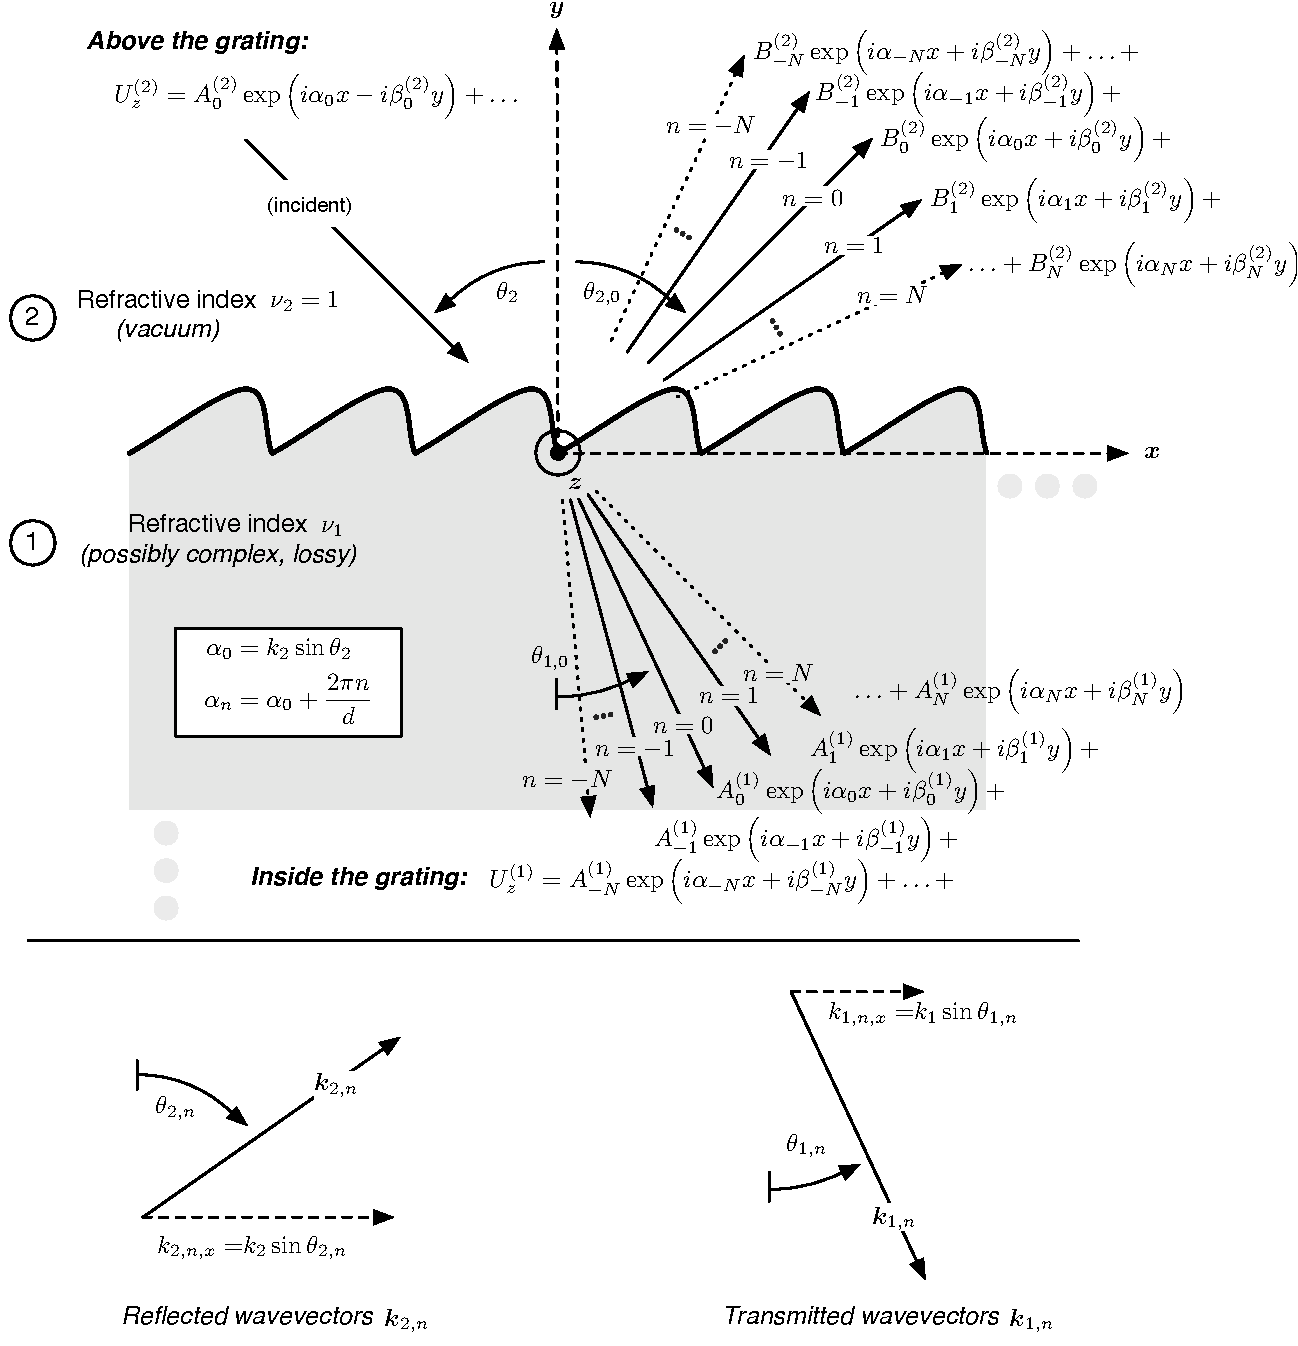
\includegraphics[scale=0.8]{../data/Chapter2/2b_rayleighExpansion/2b.pdf} 
   \caption{The Rayleigh expansion describes the electric field (TE polarization) or magnetic field (TM polarization) in homogenous media, above and below the grating.  The terms in the expansion include a finite number of propagating plane waves -- the diffraction orders -- and an infinite number of decaying, or ``evanescent'' plane waves. From the geometry of the diffracted and transmitted wave vectors, we can derive the grating equation, but we need to solve the $A_n$ and $B_n$ coefficients to determine the efficiency of each order. }
   \label{2b}
\end{figure}

The total field will have a unique solution only when the incident field $u_i$ is totally specified.  From the grating setup in Figure \ref{2a}, we know that we only have a single down-going wave, corresponding to the incident plane wave; all of the $A^{(2)}_n$ for the other propagating waves must be 0.  (We label this incident wave as $n=0$.)  We also need to reject the non-physical waves that explode as $y \rightarrow +\infty$, therefore the expansion of the field \emph{above the grating} simplifies to:
\begin{eqnarray}
u(x,y) =  A^{(2)}_0 e^{i \alpha_0 x - i \beta^{(2)}_0 y} +  \sum_{n=-\infty}^{\infty} B^{(2)}_n e^{i \alpha_n x + i \beta^{(2)}_n y}
\label{rayleighExp2}
\end{eqnarray}
The diffraction grating's reflected orders appear out of this expansion as the finite set of $n$, $\beta^{(2)}_n$, and $B^{(2)}_n$ values that create propagating plane waves travelling away from the grating.  At this point, $n$ can now be properly identified with the \emph{diffraction order}.  This is known as the \emph{Rayleigh Expansion} for the diffraction field.  (Rayleigh assumed this solution, but did not prove it, in Ref. \cite{Ray07}.)  Figure \ref{2b} shows this visually and mathematically. 

\subsubsection{Below the grating}
The field below the grating ($y<0$) can be expanded using the same  technique.  One complication is that for grating materials that absorb energy, the refractive index (and hence $k=k_1$) will be complex.\footnote{In fact, this is the case for all materials at soft x-ray wavelengths.}  In this situation there are two possibilities for the square root $\beta^{(1)}_n = \sqrt{k_1^2-\alpha_n^2}$.  The correct choice can be made by requiring that the diffracted waves remain bounded when $y\rightarrow -\infty$.  The result provides an expansion for the transmitted field, corresponding to the transmitted orders.  These are also shown visually in Figure \ref{2b}:
\begin{eqnarray}
\label{gratingEqnT}
u(x,y) =  \sum_{n=-\infty}^{\infty} A^{(1)}_{n} e^{i \alpha_n x - i \beta^{(1)}_{n} y}
\label{rayleighExp1}
\end{eqnarray}

\subsubsection{The grating equations}
These expansions for the reflected and transmitted fields show that as soon as the direction of the incident wavevector is fixed, the outgoing directions of light are determined.  For the \emph{reflected} orders, Equation \ref{rayleighExp2} gives the $x$- and $y$-components of the wavevectors:
\begin{eqnarray}
B^{(2)}_n e^{i(k_x x + k_y y)} &=& B^{(2)}_n e^{i(\alpha_n x + \beta^{(2)}_n y)} \\
k_x &=& \alpha_n \\
  &=& \alpha_0 + \frac{ 2\pi n}{d} \\
  &=& k_2 \sin \theta_2 +\frac{ 2\pi n}{d}
\end{eqnarray}
From the geometry analyzed in Figure \ref{2b}, the $x$-component of the outgoing wavevector at angle $\theta_{2,n}$ is $k_2 \sin \theta_{2,n}$.  Therefore
\begin{eqnarray}
\label{kxEqn2}
k_x &=& k_2 \sin \theta_2 +\frac{ 2\pi n}{d} = k_2 \sin \theta_{2,n}
\end{eqnarray}
and, after replacing the magnitude of the wavevector above the grating $k_2 = v_2\, \omega / c = v_2 \, 2\pi f / c =  2\pi / \lambda$, the famous grating equation (for reflected orders) is finally:
\begin{eqnarray}
\label{gratingEquation}
\frac{n \lambda}{d} = \sin \theta_{2,n} -  \sin \theta_{2}
\end{eqnarray}
(where we have assumed that $v_2 = 1$ because we are in free space, and $\lambda$ is also the free-space wavelength.) This is often called the \emph{Fraunhofer Grating Equation}.

When $n=0$, the grating equation reverts to the law of reflection ($\theta_{2,0} = \theta_2$, i.e.: the angle of reflection is equal to the angle of incidence.)  This wave corresponds to a classically-reflected wave from a normal surface.  The reflected orders that fall \emph{between} the incident wave and the $n=0$ reflection are referred to as \emph{inside orders}; using our sign convention for diffraction angles, they correspond to $n<0$.  The \emph{outside orders} ($n>0$, see Figure \ref{2b}) are diffracted at angles beyond the $n=0$ reflection.

We can also use the same technique to determine the angles of the transmitted orders.  Equation \ref{gratingEqnT} gives the $x$- and $y$-components of the transmitted wavevectors:
\begin{eqnarray}
A^{(1)}_n e^{i(k_x x + k_y y)} &=& A^{(1)}_n e^{i(\alpha_n x + \beta^{(1)}_n y)} \\
k_x &=& \alpha_n = \alpha_0 + \frac{ 2\pi n}{d} = k_2 \sin \theta_2 +\frac{ 2\pi n}{d}
\end{eqnarray}
From the geometry analyzed in Figure \ref{2b}, the $x$-component of the outgoing wavevector at angle $\theta_{1,n}$ is $k_1 \sin \theta_{1,n}$.  Therefore
\begin{eqnarray}
\label{kxEqn1}
k_x &=& k_2 \sin \theta_2 +\frac{ 2\pi n}{d} = k_1 \sin \theta_{1,n}
\end{eqnarray}
and, after again replacing $k_1$, the magnitude of the wavevector below the grating $k_1 = v_1\, \omega / c = v_1 \, 2\pi f / c =  v_1 \, 2\pi / \lambda$, the transmission grating equation is:
\begin{eqnarray}
\label{gratingEquation}
\frac{n \lambda}{d} = v_1 \, \sin \theta_{1,n} -  v_2 \, \sin \theta_{2}
\end{eqnarray}
This time, instead of checking for the law of reflection, we can check that when $n=0$, the transmission equation reverts to Snell's law of refraction ($v_1\, \sin \theta_{1,0} = v_2 \, \sin \theta_2$).

\subsubsection{Note: Simplifying $\beta_n$}
Equations \ref{kxEqn2} and \ref{kxEqn1} provide a useful simplification for $\beta_n$.  Since 
\begin{eqnarray}
k_2 \sin \theta_2 +\frac{ 2\pi n}{d} = k_2 \sin \theta_{2,n} = k_1 \sin \theta_{1,n}
\end{eqnarray}
we can go back to the expression for $\beta_n$, and easily show that 
\begin{eqnarray}
\beta_n^{(2)} &=& \sqrt{k_2^2 - \alpha_n^2} = \sqrt{k_2^2 - (\alpha_0 +2\pi n/d)^2} \\
&=& \sqrt{k_2^2 - (k_2 \sin \theta_2 +2\pi n/d)^2}\\
&=& \sqrt{ k_2^2 - (k_2 \sin \theta_{2,n})^2 }\\
&=& \sqrt{ k_2^2 (1 - \sin^2 \theta_{2,n})}\\
&=& \sqrt{ k_2^2 \cos^2 \theta_{2,n} }\\
&=& k_2 \cos \theta_{2,n}
\end{eqnarray}
Similarly, for the transmitted order,
\begin{eqnarray}
\beta_n^{(1)} &=& k_1 \cos \theta_{1,n}
\end{eqnarray}

\subsubsection{Finishing the grating problem}
Based only on Maxwell's equations and an assumption of periodicity, we have shown that a grating reflects and transmits light into a set of discrete angles.  Incredibly, this result is fully general -- it does not depend at all on the shape or nature of the grating profile; all that's required is that it be periodic.  Unfortunately, this impressive result still says nothing at all about the \emph{grating efficiency}, or the \emph{amount} of light diffracted into each order.  We still do not know anything about the \emph{amplitudes} $B_n$, $A_n$ of the diffracted plane waves, and to determine these coefficients we will need to get down and dirty inside the grooves of the grating.

Within the grooves, the wave equations (\ref{wete}, \ref{wetm}) are much more difficult to solve due to the position-dependence of $k(x,y)$.  The refractive index (and therefore the impedance $k$) will change whether inside or outside of a groove, and if the grating shape is complicated, $k(x,y)$ will be a complicated function indeed.  Several decades of intense research have produced a handful of methods for solving the full boundary-value problem, all of which are hampered by unique challenges of computational feasibility, numerical stability, and accuracy of approximations.  Table (TODO) lists the most common methods, with references and areas of applicability.   

Some methods are only applicable in specific cases.  For example, for certain particular groove profiles, there exist coordinate transformations (``conformal mappings'') which simplify the boundary conditions so they can be solved analytically.  In the following sections, we present an overview of two \emph{general} methods which can handle arbitrary groove profiles.  Before getting there, however, we take a closer look at defining grating efficiency.

\section{Defining Grating Efficiency}
In spectroscopy applications, the experimenter typically illuminates a grating with light and uses a single outgoing order ($n\neq0$) to resolve the light by wavelength.  If they are concerned about optimizing the amount of light delivered to their experiment, the ``efficiency'' question that matters to them is, ``\emph{How much light do I get out of the grating} (in the useful order), \emph{compared to how much light went in?}''  Fundamentally, this depends on how much energy is absorbed in the grating itself, and how energy is distributed between orders.

We can define the grating efficiency for a single order quite rigorously in the same way.  For electromagnetic plane waves, the \emph{Poynting Vector} represents the energy flux (or energy per unit area, W/m$^2$) carried by the wave:
\begin{eqnarray}
\vec S = \vec E \times \vec H
\end{eqnarray}
This gives the instantaneous energy flux, which will oscillate in time with the wave.  The \emph{time-averaged Poynting vector} gives the average flux delivered over a full period of the wave.  For harmonic waves, this turns out to be
\begin{eqnarray}
 \bar S  = \frac{1}{2}\, \mathbf{Re} \left( \vec E \times \vec H^\ast \right)
\end{eqnarray}
where $\vec H^\ast$ denotes the complex conjugate of $\vec H$.

We define the grating efficiency formally as \emph{the ratio of the total time-averaged Poynting flux} -- through a surface parallel to the mean grating plane -- \emph{of the outgoing order }($\bar S_n^{(2)}$) \emph{relative to the incident wave} ($\bar S^{(2)}$).  Figure \ref{2c} highlights the surface $Q_2$ used for reflected efficiencies ($e_n^{(r)}$), which spans one grating period $d$ in the $x$-direction, and has unit length in the $z$-direction.  For defining transmitted efficiencies $e_n^{(t)}$, we use a similar surface $Q_1$ at $y\leq0$.
\begin{eqnarray}
e_n^{(r)} &\equiv& \frac{\iint \limits_{Q_2} \bar S_n^{(2)} \, \hat y \, \dif z \dif x}{ \iint \limits_{Q_2} \bar S^{(2)} \, \hat y \, \dif z \dif x} \\
e_n^{(t)} &\equiv&\frac{\iint \limits_{Q_1} \bar S_n^{(1)}\, \hat y \, \dif z \dif x}{ \iint \limits_{Q_1} \bar S^{(2)}\, \hat y \, \dif z \dif x}
\end{eqnarray}
          
\begin{figure}[htbp] %  figure placement: here, top, bottom, or page
   \centering
   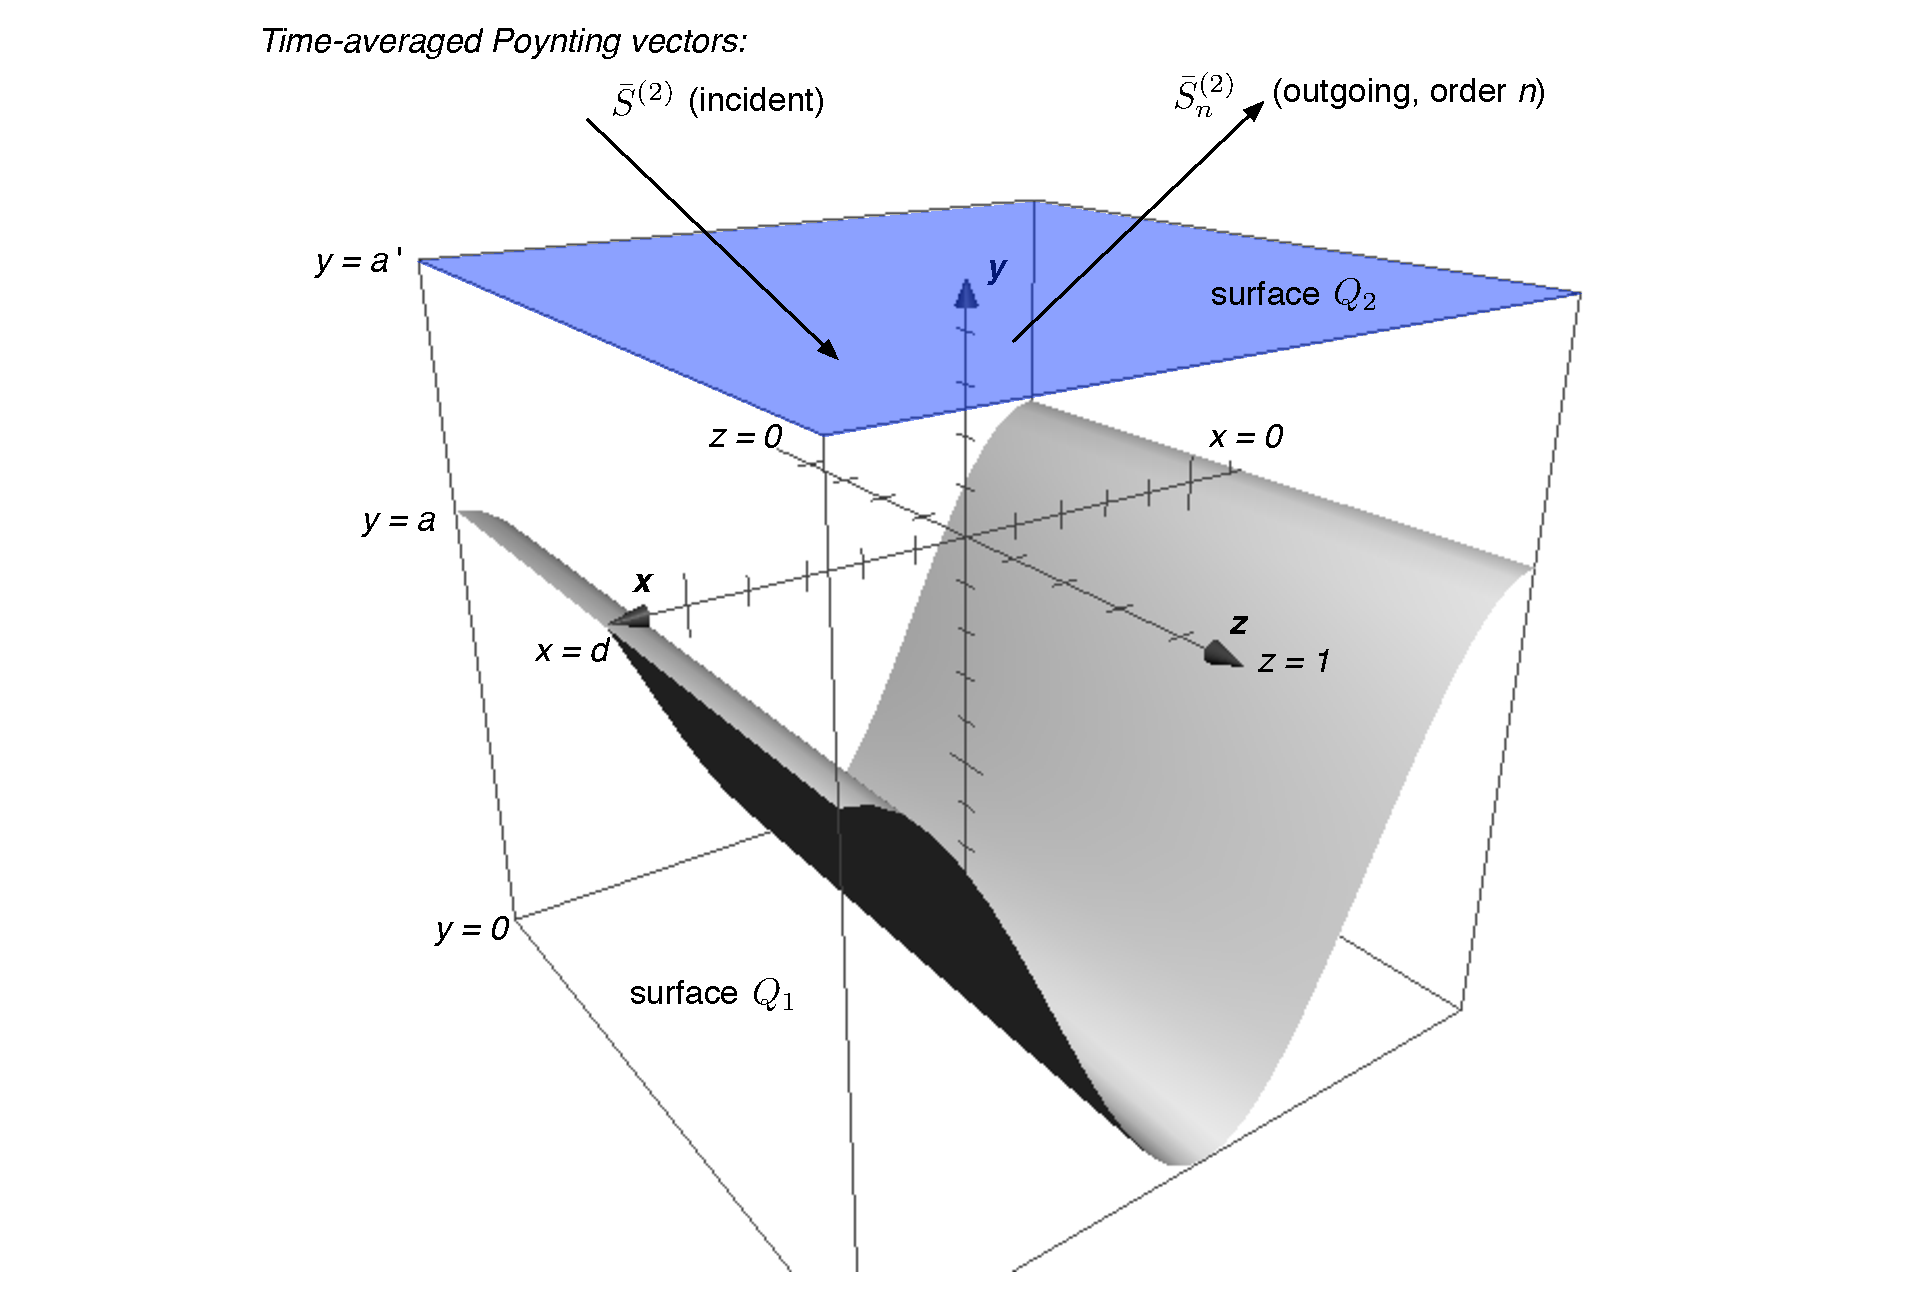
\includegraphics[scale=0.6]{../data/Chapter2/2c_poynting/2c.pdf} 
   \caption{The total electromagnetic flux through this highlighted area ($Q_2$) is used to define the grating efficiency of a diffraction order $n$, as the ratio of the flux of the diffracted wave $\bar S_n^{(2)}$ compared to the incident wave $\bar S^{(2)}$.}
   \label{2c}
\end{figure}

It turns out that this definition for efficiency can be nicely expressed in terms of the coefficients in the Rayleigh expansion for the reflected and transmitted fields (\ref{rayleighExp2}, \ref{rayleighExp1}), so that if we can solve for these coefficients, we'll have determined the grating efficiency:
\subsubsection{Reflected Efficiencies}
We know that the incident and diffracted orders are plane waves, so the magnetic field $\vec H$ is related to the electric field $\vec E$ as
\begin{eqnarray}
\left| \vec H \right| = \frac{\left| \vec E \right|}{Z_2}
\end{eqnarray}
where $Z_2 = v_2 Z_0$ is the impedance of the space above the grating (usually free space, so $v_2=1$ and $Z_2 = Z_0 = 377\Omega$, the impedance of free space). Based on the Rayleigh expansion for the outgoing field (equation \ref{rayleighExp2}), the magnitude of the time-averaged Poynting vector for the \emph{reflected order} is therefore
\begin{eqnarray}
\left| \bar S \right| = B_n^{(2)} \, B_n^{(2)\ast} \, \eta_2
\end{eqnarray}
where we have defined \fbox{$\eta_2 \equiv 1/(2Z_2)$} in the case of TE polarization, and \fbox{$\eta_2 \equiv 2Z_2$} for TM polarization.  The direction of the vector is along the propagation direction, i.e.: at an angle $\theta_{2,n}$ to the $y$-axis, therefore the integrated flux through the surface is:
\begin{eqnarray}
\iint \limits_{Q_2} \bar S_n^{(2)} \, \hat y \, \dif z \dif x &=& \int \limits_0^d \int \limits_0^1 \bar S_n^{(2)} \, \hat y \, \dif z \dif x \\
&=& B_n^{(2)} \, B_n^{(2)\ast} \, \eta_2 \, d \cos \theta_{2,n} 
\end{eqnarray}
For the incident wave, the integrated flux is similarly 
\begin{eqnarray}
\iint \limits_{Q_2} \bar S^{(2)} \, \hat y \, \dif z \dif x = A_0^{(2)} \, A_0^{(2)\ast} \, \eta_2 \, d \cos \theta_{2} 
\end{eqnarray}
and so the reflected efficiency in order $n$ is:
\begin{eqnarray}
e_n^{(r)} &=& \frac{    B_n^{(2)} \, B_n^{(2)\ast} \cos \theta_{2,n}       }{    A_0^{(2)} \, A_0^{(2)\ast}  \cos \theta_{2}     }
\end{eqnarray}
We can simplify this somewhat by choosing a unit amplitude for the incident field, i.e.: $A_0^{(2)} = 1$V/m for the TE electric field, or 1A/m for the TM magnetic field. Also, since $\beta_n^{(2)} = k_2 \cos \theta_{2,n}$, we can simplify this to
\begin{eqnarray}
e_n^{(r)} &=& B_n^{(2)} \, B_n^{(2)\ast} \, \frac{     \beta_n^{(2)}       }{    \beta_0^{(2)}      }
\end{eqnarray}

\subsubsection{Transmitted Efficiencies}
Gratings used in the soft x-ray regime are always used in reflection, due to the high absorption of materials at these wavelengths.  However, since we're working on a general theory with application to all gratings, we can go through the same process for simplifying the transmitted efficiencies.  

Again, we define \fbox{$\eta_1 \equiv 1/(2Z_1)$} in TE polarization, and \fbox{$\eta_1 \equiv 2Z_1)$} in TM polarization, where $Z_1 = v_1 Z_0$ is the impedance of the grating substrate material.  The same integrations over the surface $Q_1$ give the ratio between the total transmitted and incident fluxes:
\begin{eqnarray}
e_n^{(t)} &=& \frac{    A_n^{(1)} \, A_n^{(1)\ast} \cos \theta_{1,n} \, \eta_1       }{    A_0^{(2)} \, A_0^{(2)\ast}  \cos \theta_{2} \,  \eta_2   }
\end{eqnarray}
In this case, the difference in impedance above and below the grooves causes $\eta_1$ and $\eta_2$ to remain in the formula, so the final simplification depends on polarization:
\begin{eqnarray}
e_n^{(t)} =& A_n^{(1)} \, A_n^{(1)\ast} \frac{  \beta_n^{(1)}   } {  \beta_0^{(2)} }  & \textrm{(TE Polarization)} \\
=& A_n^{(1)} \, A_n^{(1)\ast} \frac{  \beta_n^{(1)}   } {  \beta_0^{(2)} }  \left( \frac{v_2}{v_1} \right)^2 & \textrm{(TM Polarization)}
\end{eqnarray}


                         
\section{Solving for efficiency}


          - Solving: Requires periodic representation of refractive index: only true at fixed (y).  Needs computational methods
          
          -- key set of differential equations to solve... d2En/dy2 + k2 En = 0
\subsection{Numerical Challenges}
\subsubsection{Integration of growing exponentials}
               - Integrating growing exponentials: floating point rounding error leads to runaway [reference: Neviere: S-matrix; Somebody: R-matrix]
\subsubsection{Truncation of Fourier expansions}
               - Must truncate Fourier expansion.  Problem in TM case: makes field discontinuous, where should be continuous. [reference: Li, FFF]
\subsection{Applying boundary conditions within the groove region}
          - Highlighted methods for dealing with boundary conditions in groove region:
          
               - RCWA: split into thin layers and make rectangular
               
               - Differential method
               
          - Table of methods, areas of applicability, and references
          
\subsection{Handling stacks of gratings}
\label{stacksOfGratings}
\begin{figure}[htbp] %  figure placement: here, top, bottom, or page
   \centering
   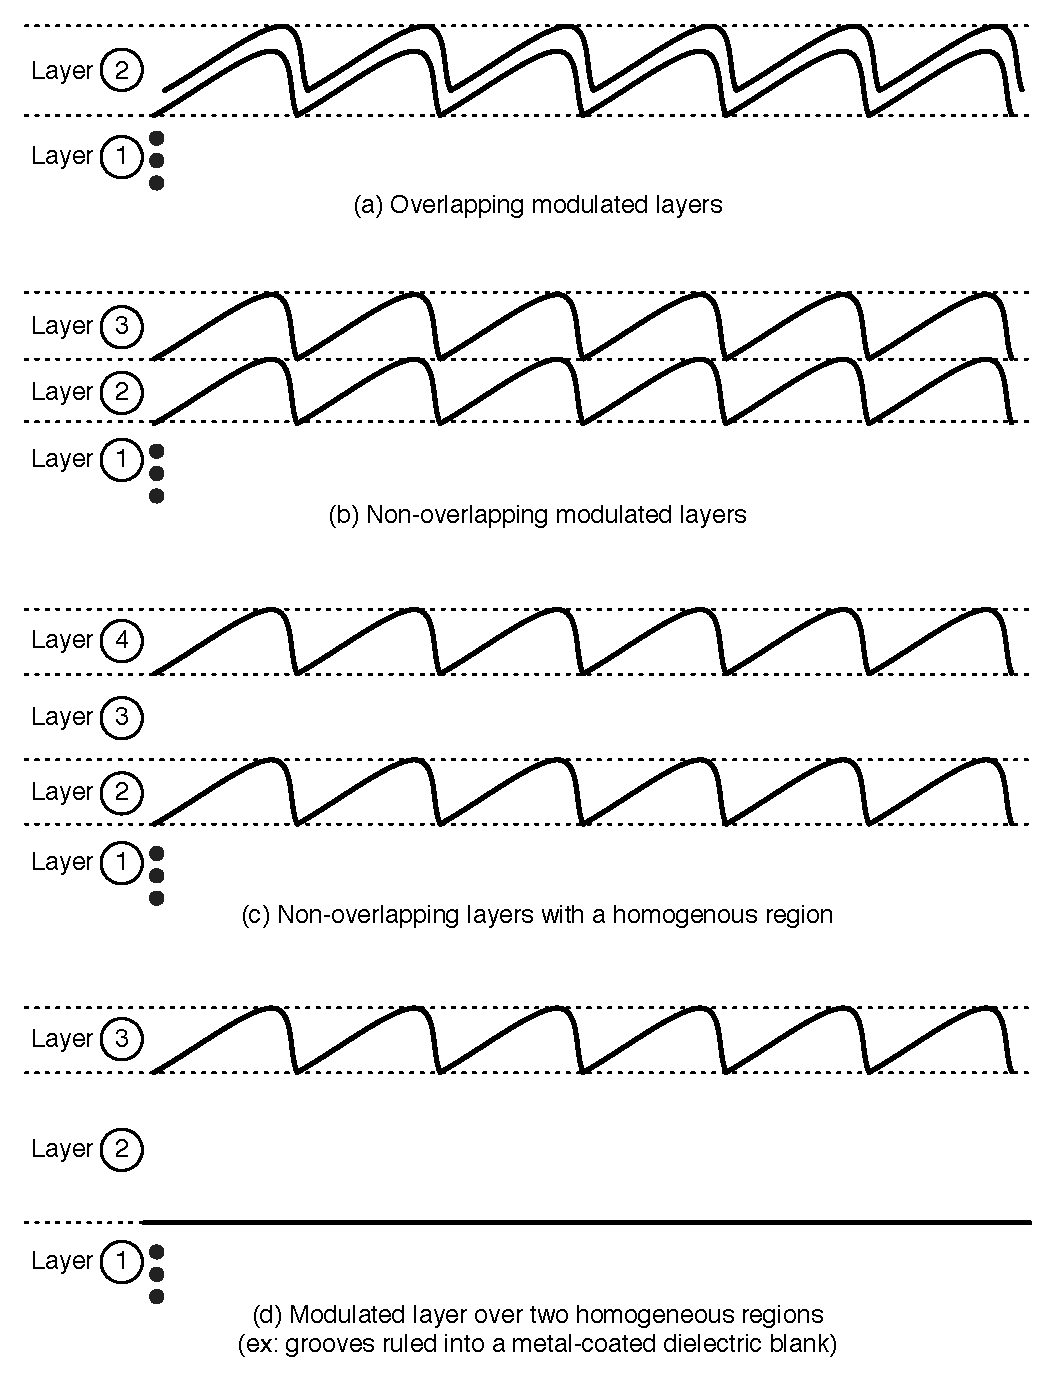
\includegraphics[scale=0.8]{../data/Chapter2/2d_stacksOfGratings/2d_1.pdf} 
   \caption{Arbitrarily-complicated structures can be handled by dividing the grating into layers, where each layer is either homogenous (constant refractive index), or modulated (with a refractive index that changes periodically as a function of $x$ at any given height $y$).}
   \label{2d-1}
\end{figure}


\begin{figure}[htbp] %  figure placement: here, top, bottom, or page
   \centering
   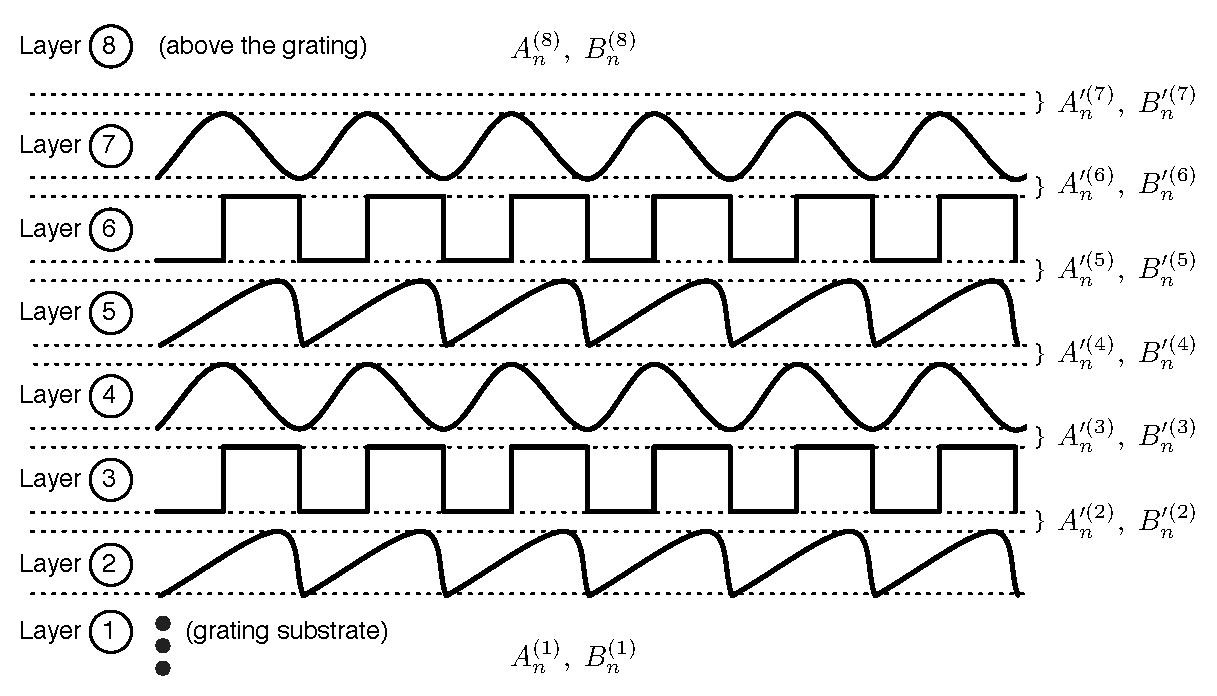
\includegraphics[scale=0.8]{../data/Chapter2/2d_stacksOfGratings/2d_2.pdf} 
   \caption{Modulated layers in a complicated stack of gratings.  In between every layer, we can insert an imaginary, infinitely-thin homogenous layer where the Rayleigh expansion applies.  The $A^{\prime}_n$ and $B^{\prime}_n$ expansion coefficients connect the boundary conditions between layers.  Within each layer, the Rayleigh expansion does not apply -- inside the grooves, the field cannot be represented as a simple sum of plane waves -- and numerical methods are required to approximate it.}
   \label{2d-2}
\end{figure}


\section{X-rays and materials: how do they interact?} (Especially: lossy metals)
          - Characterized: atomic scattering factor -> *complex refractive index*
          
          FIGURE 2e: plot of real and imaginary components... Metals at 100-1000eV.
          
          - RI Derived from Henke Data
          
               - Reference CXRO calculator
               
          - Note: total external reflection (overcome notoriously absorbing materials via grazing incidence)


Next chapter: look at the how this is applied, and what we can learn about grating efficiency using the theory

REMAINING QUESTIONS: numerical integration of WHAT.  (A: 2nd order in TE; 1st-order in TM.  Eqn II.2')

	How to get coefficients for k2(x,y)?
	